\documentclass[10pt]{article} 
\usepackage[T1]{fontenc} 
\usepackage[utf8]{inputenc}
\usepackage{geometry} 
\geometry{verbose,marginparwidth=0.5in,tmargin=1in,bmargin=1in,lmargin=1in,rmargin=1in} 
\usepackage{lmodern}

\usepackage{booktabs}

\usepackage{enumitem}
% \setlist{nosep}

% \usepackage{amsfonts}
% \usepackage{amsmath}
\usepackage{comment}
\usepackage{listings}
\usepackage{mathtools}
\usepackage{bbm}
\newcommand{\one}{\mathbbm{1}}



\begin{document}


\begin{center}
\textbf{Econ 512}

\emph{Fall 2018}\\[1em]

Solution to Homework 1 -- Introduction/Review of Matlab Basics\\
Yuanxing Long\\
\end{center}

\bigskip 

\noindent
\textbf{1.} The matlab codes are given by: 
\begin{lstlisting}
X=[1 1.5 3 4 5 7 9 10];
Y1=-2+0.5*X;
Y2=-2+0.5*X.^2;
figure
plot(X,Y1,'*',X,Y2,'*')
\end{lstlisting}
The relationships between X and Y1, Y2 are plotted as: \\
 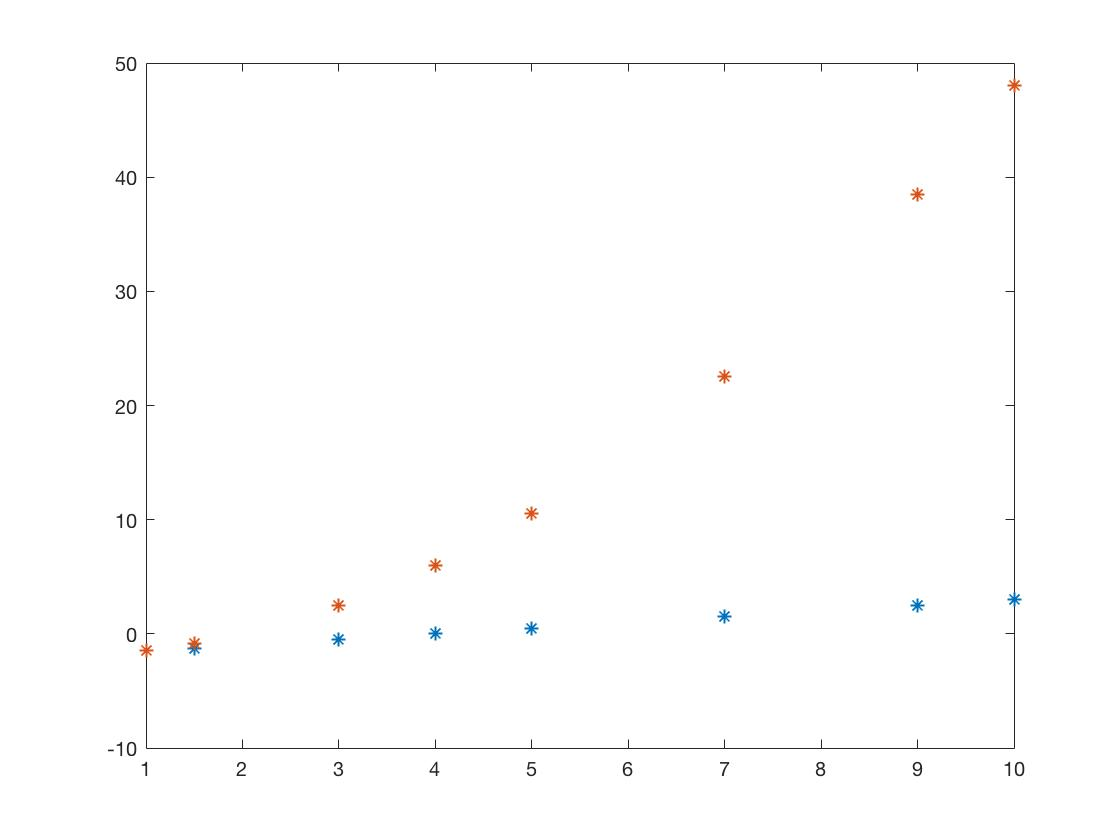
\includegraphics[scale=0.2]{hw1q1.jpg}\\ 
 The blue stars are for $Y1$ and the red stars for $Y2$.


\bigskip 

\noindent
\textbf{2.} The matlab codes are given by: 
\begin{lstlisting}
step=(20-(-10))/199;
X_2=-10:step:20;
s=sum(X_2)
\end{lstlisting}
The output which is the sum of the elements of generated vector is 1000.\\



\bigskip 

\noindent
\textbf{3.} The matlab codes are given by:
\begin{lstlisting}
A=[2, 4, 6; 
    1, 7, 5; 
    3, 12, 4];
b=[-2; 3; 10];
C=A'*b
D=(A'*A)\b
E=sum(A)
F=A([1,3],1:2)
x=A\b
\end{lstlisting}
The output are: $C$=$ % 
\begin{bmatrix}
29 \\
133\\
43 \\ %
\end{bmatrix} % 
$,
$D$=$ % 
\begin{bmatrix}
-3.2505 \\
0.3961 \\
0.8037 \\ %
\end{bmatrix} % 
$,
$E=205$,
$F$=$ % 
\begin{bmatrix}
2 & 4  \\
3 & 2  \\  %
\end{bmatrix} % 
$ and the solution to $Ax=b$ is $x$=$ % 
\begin{bmatrix}
-0.1622 \\
 1.2432\\
-1.1081\\ %
\end{bmatrix} % 
$. 

\bigskip

\noindent
\textbf{4.} The matlab codes are given by:
\begin{lstlisting}
I=eye(5);
B=kron(I, A)
\end{lstlisting}
We use kronecker product to generate matrix B. 


\bigskip 

\noindent
\textbf{5.}  The matlab codes are given by:
\begin{lstlisting}
A5= normrnd(10,5,5,3)
A5(A5<10)=0;
A5(A5>=10)=1;
disp(A5)
\end{lstlisting}
We use 'normrnd' to generate the matrix A and then convert it a new matrix by the above codes. 


\bigskip

\noindent
\textbf{6.}  The matlab codes are given by:
\begin{lstlisting}
M = csvread('datahw1.csv');
save('datahw1.mat','M');
load('datahw1.mat');
x1 =  M(:,3); % export
x2 = M(:,4);  % RD
y = M(:,5);  % prod
x3 = M(:,6); % capital
X=[x1 x2 x3];
% Since the matlab does not have a OLS regression function for multivariate
% regression that returns both the coefficients and their standard errors,
% I use a new function to find it. 
[b_hat, se]= ols(y, X, 1)
\end{lstlisting}

The reported estimates and heteroskedastic standard errors are:\\
$\hat{\beta}_1$ =0.0817 , $\hat{\beta}_2$ =0.1201, $\hat{\beta}_3$ =0.1399, $\hat{\beta}_4$ =0.0295\\
$se(\hat{\beta}_1)$ =0.0193, $se(\hat{\beta}_2)$ =0.0061, $se(\hat{\beta}_3)$ =0.0089, $se(\hat{\beta}_4)$ =0.0020. \\\\
The function $ols$ is given below:
 \begin{lstlisting}
function[b_hat, se] = ols(Y, X, hetero)
% Y - dependent variable
% X - regressors (without a constant)
% hetero - 1 if using heteroskedasticity and 0 if using homoskedisticity
    [n, ~] = size(X);

    if numel(Y) ~= n
        error('Incompatible data.') 
    end
    
    % Get estimates
    X1 = [ones(n, 1) X]; XX1 = X1' * X1;
    b_hat = XX1 \ (X1' * Y);
    r_hat = Y - X1 * b_hat;
    
    % Get asyvar.
    switch hetero
        case 1
            X2 = bsxfun(@times, X1, r_hat);
            avar = XX1 \ (X2' * X2) / XX1;
        otherwise
            avar = (r_hat' * r_hat) * inv(XX1) / n; 
    end
 
    se = sqrt(diag(avar));
    
end
\end{lstlisting}

\bigskip 
\textbf{Output file}
\begin{lstlisting}
Econ512_HW1

s =

        1000


C =

    29
   133
    43


D =

   -3.2505
    0.3961
    0.8037


E =

   205


F =

     2     4
     3    12


x =

   -0.1622
    1.2432
   -1.1081


B =

     2     4     6     0     0     0     0     0     0     0     0     0     0     0     0
     1     7     5     0     0     0     0     0     0     0     0     0     0     0     0
     3    12     4     0     0     0     0     0     0     0     0     0     0     0     0
     0     0     0     2     4     6     0     0     0     0     0     0     0     0     0
     0     0     0     1     7     5     0     0     0     0     0     0     0     0     0
     0     0     0     3    12     4     0     0     0     0     0     0     0     0     0
     0     0     0     0     0     0     2     4     6     0     0     0     0     0     0
     0     0     0     0     0     0     1     7     5     0     0     0     0     0     0
     0     0     0     0     0     0     3    12     4     0     0     0     0     0     0
     0     0     0     0     0     0     0     0     0     2     4     6     0     0     0
     0     0     0     0     0     0     0     0     0     1     7     5     0     0     0
     0     0     0     0     0     0     0     0     0     3    12     4     0     0     0
     0     0     0     0     0     0     0     0     0     0     0     0     2     4     6
     0     0     0     0     0     0     0     0     0     0     0     0     1     7     5
     0     0     0     0     0     0     0     0     0     0     0     0     3    12     4


A5 =

   24.5400    8.6377    8.2308
   14.1261   15.4921    5.8821
   16.8949    8.6106    2.1147
    4.7091   13.5077   12.5399
    7.6569   -0.2591   11.4099

     2     4     6
     1     7     5
     3    12     4


b_hat =

    0.0817
    0.1201
    0.1399
    0.0295


se =

    0.0193
    0.0061
    0.0089
    0.0020

\end{lstlisting}



\end{document}
